\section{The cube}
\label{sec:cube}

In this section we construct sources for the unit cube $[-\tfrac12,\tfrac12]^3$ at $k = 2\pi$, so that the side is one wavelength. By \autoref{thm:skeleton} the sources belong on the twelve bisector planes of the edges, and they must resolve current densities that are singular at the edges and vertices. We describe the layout of the sources, the singular tail that continues them towards the edges, and the boundary points, and then present the results.

\subsection{Sources on the skeleton}
\label{sec:cubelayout}

The layout has three kinds of free sources (\autoref{fig:cubelayout}).

\emph{Base points.} A grid of $n_b\times n_b$ electric dipoles on each face of an inner cube at depth $0.2$ below the faces represents the smooth part of the field. These points stand for the inner part of the skeleton, whose field is smooth outside the inner cube.

\emph{Edge lines.} For each edge we choose depths that decrease geometrically,
\begin{equation}
  d_j = 0.2\,q^{\,j}, \qquad j = 0,1,\dots, \qquad \text{down to } d_J = 0.2\cdot 2^{-J},
  \label{eq:depths}
\end{equation}
and place at each depth a line parallel to the edge, on the bisector plane, at depth $d_j$ below the two faces. We call $J$ the level of the layout. We use two ratios: $q = 1/2$, which gives one line per octave of depth, and $q = 2^{-1/2}$, which gives two.

A lightning solver in two dimensions places one point source at each depth \cite{gopal2019siam}. In three dimensions a row of points at depth $d$ would need about $1/d$ of them, so we let each line carry a continuous dipole density instead. With $t$ the coordinate along the line at depth $d$, the stretched variable
\begin{equation}
  u(t) = \frac{1}{\lambda}\log\frac{\tfrac12+t}{\tfrac12-t}, \qquad \lambda = \log\frac{1-d}{d},
\end{equation}
maps the line to $[-1,1]$ and resolves every scale between $d$ and the length of the edge near both vertices. The density is a vector polynomial in $u$ with $n = n_0 + \lceil 2\log(1/d)\rceil$ Legendre modes, and each line exists twice, once with electric and once with magnetic dipoles. A line at depth $10^{-3}$ thus costs about $25$ modes, where a row of points would need a thousand. On the cube the method is therefore no longer free of integration, but the integrals are one-dimensional, and they are evaluated by a quadrature that shares its nodes between the boundary points (\autoref{app:lines}).

\emph{Vertex points.} On the body diagonal through each vertex we place an electric and a magnetic point dipole at each of the same depths.

\begin{figure}[htbp]
  \centering
  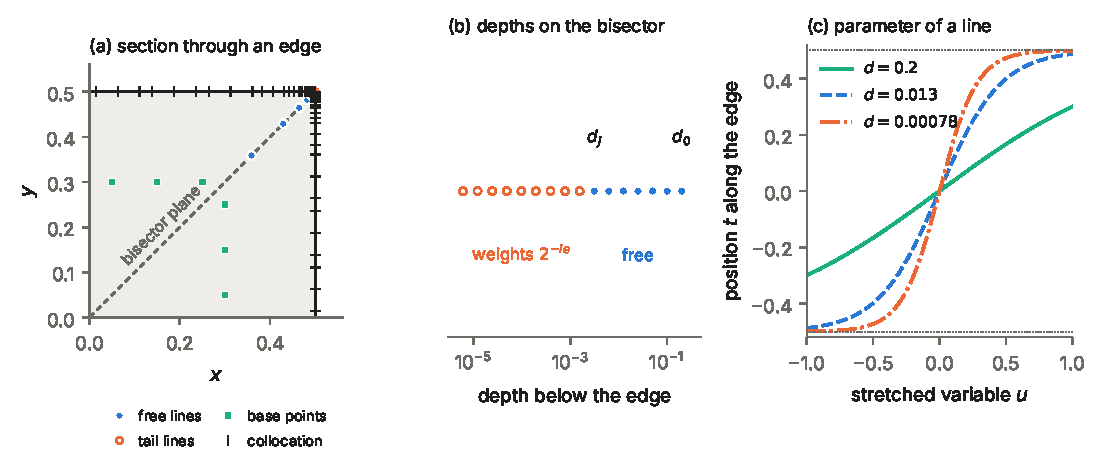
\includegraphics[width=0.8\textwidth]{fig_cube_layout.pdf}
  \caption{Source layout of the cube. (a) Cross-section through the middle of an edge: the lines, seen end on, sit on the bisector plane at the depths \eqref{eq:depths}; base points lie on an inner cube; boundary points on the two faces are graded towards the edge. (b) The depths on a logarithmic scale: free lines down to $d_J$, then the tail with fixed weights. (c) The stretched variable $u$ along a line, which clusters the modes towards the two vertices as the depth decreases.}
  \label{fig:cubelayout}
\end{figure}

\subsection{The singular tail}
\label{sec:tail}

The deepest free line lies at the depth $d_J$. The current sheet of \autoref{thm:skeleton} continues below this depth, all the way to the edge, and cutting it off leaves an error that decays only like $d_J^{0.55}$ in our experiments. To continue the free lines to ever smaller depths would be expensive, and it is not necessary, because close to the edge the form of the currents is known.

We therefore continue the lines at the depths $d_J2^{-i}$, $i = 1,\dots,9$, without new unknowns. These lines are not free: they carry the modes of the line at $d_J$, multiplied by the fixed weights $2^{-ie}$. We call this continuation the \emph{singular tail}. The exponent $e$ is not fitted. It follows from the edge expansion of the field, as we now show.

Consider one edge of the cube, with the coordinate $s$ along the edge and polar coordinates $(\rho,\phi)$ around it, so that the exterior is the wedge $0<\phi<3\pi/2$. Near the edge the field is a sum of terms of two types \cite{meixner1972,costabel2000},
\begin{align}
  E_s &= a_n(s)\,\rho^{2n/3}\sin(2n\phi/3), & n &= 1,2,\dots, \label{eq:tm}\\
  H_s &= b_n(s)\,\rho^{2n/3}\cos(2n\phi/3), & n &= 0,1,2,\dots, \label{eq:te}
\end{align}
each multiplied by a power series in $\rho^2$. The transverse components follow from $E_s$ and $H_s$ and are one power of $\rho$ lower.

The reflection used in the proof of \autoref{thm:skeleton} continues each term into the body by the same formula. The two continuations, through the two faces, meet on the bisector half-plane, which is the wall of the skeleton at this edge. With the angle $\psi = \phi - 3\pi/4$ measured from the exterior bisector, the wall is $\psi = \pi$ seen from one side and $\psi = -\pi$ from the other. The angular factors in \eqref{eq:tm} and \eqref{eq:te} are sines and cosines of $2n\psi/3$. Their jump across the wall is proportional to $\sin(2n\pi/3)$ for the part that is odd in $\psi$ and vanishes for the even part. Terms with $n$ a multiple of three do not jump: they are polynomial fields and need no sources.

Let $m$ be the mirror in the bisector plane. A term is even under $m$ if $E_s$ is even in $\psi$ or $H_s$ is odd in $\psi$. For an even term the tangential electric field is continuous across the wall and the tangential magnetic field jumps, so by \eqref{eq:jumps} it leaves only an electric current. An odd term leaves only a magnetic current. Reading off the leading jumps gives the current densities of \autoref{tab:edgeexp}, where $\rho$ is now the depth on the wall. The electric current behaves like $\rho^{-1/3}$ along the edge and like $\rho^{2/3}$ along the bisector, and the magnetic current like $\rho^{1/3}$ and $\rho^{4/3}$.

It remains to turn the densities into weights. The tail replaces the current sheet below $d_J$ by lines at the depths $d_J2^{-i}$, and a line stands for the strip of the sheet around it, whose width is proportional to its depth. A density $\rho^{e-1}$ therefore gives the line weights $2^{-ie}$, with $e = 2/3$, $5/3$, $4/3$ and $7/3$ for the four components.

\begin{table}[htbp]
  \centering
  \caption{Exponents of the edge tail of the cube. The current density on the bisector half-plane behaves like $\rho^{e-1}$ at depth $\rho$ below the edge.}
  \label{tab:edgeexp}
  \begin{tabular}{llll}
    \toprule
    Current & Component & Density & Tail exponent $e$ \\
    \midrule
    electric, $J_s = [H_\rho]$ & along the edge & $\rho^{-1/3}$ & $2/3$ \\
    electric, $J_\rho = [H_s]$ & along the bisector & $\rho^{2/3}$ & $5/3$ \\
    magnetic, $K_s = [E_\rho]$ & along the edge & $\rho^{1/3}$ & $4/3$ \\
    magnetic, $K_\rho = [E_s]$ & along the bisector & $\rho^{4/3}$ & $7/3$ \\
    \bottomrule
  \end{tabular}
\end{table}

The vertex points are continued in the same way along the diagonal. Near a vertex the field behaves like $r^{\nu-1}$ in the distance $r$, and the tail weights of the electric and magnetic dipoles have the exponents $\nu+2$ and $\tau+2$, where $\nu = 0.4542$ and $\tau = 0.840$ are the smallest electric and magnetic exponents of the corner. We computed them from eigenvalue problems on the sphere (\autoref{app:cone}), and they agree with the values $0.45410$ and $0.84108$ of De Smedt and Van Bladel \cite{desmedt1986}.

The tails are cheap: at $J = 8$ all of them together are $9\%$ of the unknowns. \autoref{fig:edgeresidual} shows their effect on the residual at the boundary. Without the tail the residual is of order one at all distances from the edge below $d_J$. With the tail it stays near $10^{-2}$ or below down to the end of the tail at $d_J2^{-9}$, so the strip in which the boundary condition is violated is narrower by a factor of $2^{9}$.

\begin{figure}[htbp]
  \centering
  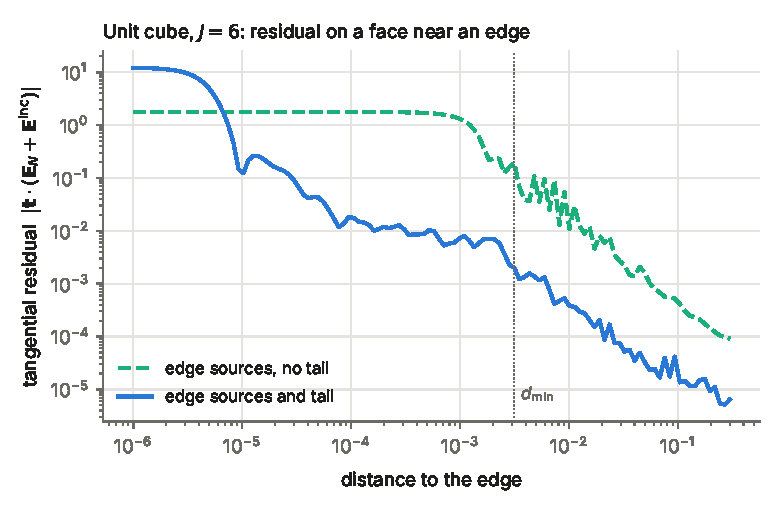
\includegraphics[width=0.6\textwidth]{fig_edge_residual.pdf}
  \caption{Unit cube, $J = 6$, one depth per octave: tangential residual on a face as a function of the distance to an edge, away from the vertices, with and without the tail. The dotted line marks the deepest free depth $d_J$.}
  \label{fig:edgeresidual}
\end{figure}

\subsection{Boundary points, weights and symmetry}

The boundary points on each face form a tensor grid. In each direction the nodes are Gauss--Legendre points on panels that halve in length towards both edges until they are shorter than $d_J$, and panels in the interior are no longer than $h_{\max}$. We use three nodes per panel for $q = 1/2$ and four for $q = 2^{-1/2}$. The fit needs enough equations at every scale: with two nodes per panel and $q = 1/2$ the error at $J = 5$ is $85\%$, although the residual at the boundary points is small.

The rows are weighted by $w_i = A_i\,\rho_i$, where $A_i$ is the area represented by the point and $\rho_i$ its distance to the nearest edge, so that the fit does not spend its effort on the edge singularity of the residual. All resolution parameters grow together with the level: $n_0 = \max(4, 2J-4)$, and $(n_b, h_{\max}) = (4, 0.25)$ for $J\le5$ and $(6, 0.15)$ for $J\ge6$.

The cube and the layout are symmetric under the three mirrors $x\to-x$, $y\to-y$ and $z\to-z$. Any incident field is the sum of eight parts of definite parity, and each part needs only the sources and boundary points of one octant. The eight matrices are signed sums of the same reflected blocks, so the line integrals are computed once, and the factorisation of a class serves every incident wave. Our standard wave excites two classes, and a general wave excites all eight.

\subsection{Results}
\label{sec:cuberesults}

\autoref{tab:cube} lists the results for both depth ratios, and \autoref{fig:cubeconv} shows them against the number of unknowns. Since the cube has no exact solution, the reference is the finest layout, with two depths per octave at level $J = 11$. We first describe the convergence and then the evidence that the limit is the correct field.

\begin{table}[htbp]
  \centering
  \caption{Unit cube, $k = 2\pi$. MFS with edge sources and tails, with one and with two source depths per octave: unknowns and equations per parity class (two classes are solved), wall time, difference from the run with two depths per octave at $J = 11$, and optical mismatch.}
  \label{tab:cube}
  \small
  \begin{tabular}{lrrrrll}
    \toprule
    Depths & $J$ & Unknowns & Equations & Time [s] & Error & Optical \\
    \midrule
\tablebody{cube_mfs_short}
    \bottomrule
  \end{tabular}
\end{table}

With two depths per octave the error falls from $5.1\times10^{-3}$ at $J = 4$ to $1.5\times10^{-5}$ at $J = 10$, by a factor of $2.4$ to $3.5$ per level, and the optical mismatch falls with it to $1.8\times10^{-6}$. Let $N$ be the number of unknowns of the whole cube, which is eight times the entry of \autoref{tab:cube}. Against $\sqrt{N}$ the errors lie on a straight line (\autoref{fig:cubeconv}),
\begin{equation}
  \varepsilon \approx 0.44\,\exp\bigl(-0.048\sqrt{N}\bigr),
  \label{eq:rootexp}
\end{equation}
to within a factor of $1.3$ over two and a half orders of magnitude. This is the root-exponential convergence of the lightning solvers in two dimensions \cite{gopal2019siam}, and it is what the layout suggests: both the number of lines and the number of modes per line grow linearly with the level, and the error decays geometrically with the level. Measured as an algebraic order, the rate rises from about $N^{-2.5}$ to $N^{-6}$ along the table.

\begin{figure}[htbp]
  \centering
  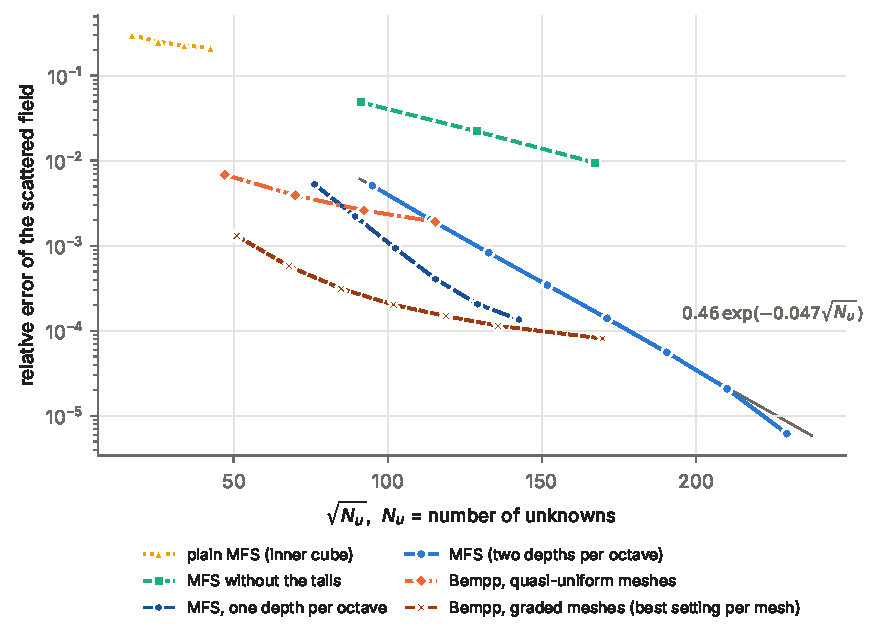
\includegraphics[width=0.78\textwidth]{fig_cube_convergence.pdf}
  \caption{Unit cube, $k = 2\pi$: error of the scattered field against the square root of the number of unknowns $N$ of the whole cube (for the MFS, all eight parity classes together). The grey line is the fit \eqref{eq:rootexp} to the layout with two depths per octave. For Bempp the smallest error over all settings is shown for each mesh.}
  \label{fig:cubeconv}
\end{figure}

The layout with one depth per octave has about $60\%$ of the unknowns and takes between $30\%$ and $60\%$ of the time. Down to level $J = 7$ its errors equal those of the denser layout to within $20\%$, and then it stalls near $1.5\times10^{-4}$. The matrices are well conditioned, so this is not an effect of rounding. The two-dimensional analogue behaves in the same way: for the unit square with point sources on the bisectors of the corners, the error of the far field stalls at $8\times10^{-5}$ for $q = 1/2$, at $6\times10^{-6}$ for $q = 0.6$ and at $10^{-9}$ for $q = 2^{-1/2}$. We therefore regard $q = 1/2$ as the economical choice for errors down to $2\times10^{-4}$ and $q = 2^{-1/2}$ as the choice below.

The tails are essential for this convergence. With the same edge lines but without the tails, the error is $5.4\times10^{-2}$, $2.5\times10^{-2}$ and $1.1\times10^{-2}$ for $J = 4$, $6$ and $8$, so at $J = 8$ the tails reduce the error by a factor of $64$. The exponents matter as well. Adding the next term of each edge expansion to the tail changes the error by less than $1\%$ of its value, but lowering the exponents of the two transverse components by one gives an error of $65\%$.

Three checks support the reference. First, the result is insensitive to the parameters of the layout: at $J = 9$ the field changes by less than $3\times10^{-6}$ when the modes, the tails, the base grid or the boundary grid are refined. Second, a run at $J = 12$ with a finer interior grid ($n_b = 8$, $h_{\max} = 0.1$) differs from the reference by $7\times10^{-6}$ and has an optical mismatch of $9\times10^{-7}$. Third, we computed the same field with Bempp on meshes graded towards the edges. With $10368$, $14112$, $18432$ and $28800$ unknowns the boundary element field differs from the MFS reference by $2.0\times10^{-4}$, $1.5\times10^{-4}$, $1.1\times10^{-4}$ and $8\times10^{-5}$, and its extrapolated extinction cross-section is $2.92786$, where the MFS gives $2.92798$. The two methods thus agree to $8\times10^{-5}$ in the field and to $4\times10^{-5}$ in the cross-section. Below that level the only reference for the MFS is its own convergence.

%%OTHERCASES%%
